\section{Ejercicio B - Método de Romberg}


\subsection{Problema}

Utilizando los resultados del apartado a), realice la extrapolación de Romberg para obtener una mejor aproximación numérica de las dos integrales de Fresnel. Indique cuántas evaluaciones de las funciones se requieren.


\subsection{Análisis}


\subsubsection{Extrapolación de Richardson}

La extrapolación de Richardson es un método que pertenece a la familia de aceleración de series.

Se puede aplicar cuando el error de una aproximación sigue la forma: 

$$
O(x^p) = \sum_{k=p} a_k (x - c)^k
$$

Dada una constante que nos interesa aproximar, como por ejemplo:

$$
m = \int_{a}^{b}  f(x) dx
$$

planteamos una aproximación $L_p(h)$, donde $h$ es el tamaño del paso en que dividimos $I = [a, b]$. Le daremos la forma: 

$$
m = L_p(h) + \sum_{k} a_k h^k
$$

El error es de orden $O(h^p)$.

	Si reducimos el paso por un factor de $\frac{h}{q}$ y manipulamos algebraicamente obtenemos una nueva aproximación $L_{p+1}$ en que el error es de orden $O(h^{p+1})$.


\subsubsection{Método de Romberg}

El método de romberg se basa en combinar la regla compuesto del trapecio con la extrapolación de Richardson para obtener una mejor aproximación a integrales que si se usara solamente la regla compuesta del trapecio.

\subsubsection{Implementación}

La implementación del método se puede ver en \ref{code:romberg}

\subsection{Resolución}


El código que resuelve el ejercicio se puede ver en \ref{code:ex2}. 

\paragraph{Valores} Los resultados se han compilado en una tabla (para un valor de $m= 8$).


\begin{table}[H]
	\centering
	\csvreader[
	tabular=|l|l|l|,
	table head=\hline \textbf{fn} & \textbf{Valor} & \textbf{Num. Evals} \\\hline,
	late after last line=\\\hline,
	]{data/romberg_c_s.csv}{}{\csvlinetotablerow}
\end{table}

En la siguiente figura podemos ver como el método de Romberg converge con $m > 5$.

\begin{figure}[h!]
	\centering
	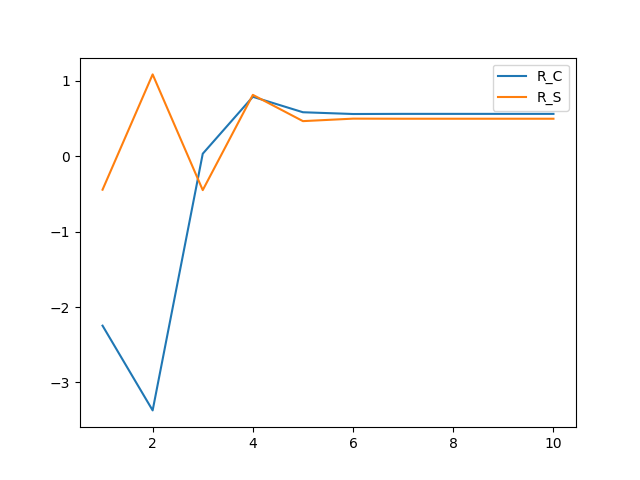
\includegraphics[width=\linewidth]{figures/romb_for_m.png}
	\caption{Método de Romberg según incrementamos $m$.}
	\label{fig:romb_for_m}
\end{figure}
